\documentclass[10pt,a4paper]{article}

\usepackage[a4paper, top=22mm, bottom=22mm, left=20mm, right=20mm]{geometry}
\usepackage{tikz}
\usetikzlibrary{shapes.geometric,arrows.meta,positioning,fit,
                backgrounds,calc,automata}
\usepackage{booktabs}
\usepackage{array}
\usepackage{tabularx}
\usepackage{multirow}
\usepackage{xcolor}
\usepackage{colortbl}
\usepackage{enumitem}
\usepackage{titlesec}
\usepackage{fancyhdr}
\usepackage{amsmath}

\usepackage{parskip}
\usepackage{hyperref}
\usepackage{caption}
\usepackage{pifont}
\usepackage{makecell}

%% ── colours ─────────────────────────────────────────────────────────────────
\definecolor{ruleclr}{RGB}{180,180,180}
\definecolor{hdrclr}{RGB}{20,20,20}
\definecolor{cellbg}{RGB}{235,235,235}
\definecolor{altbg}{RGB}{250,250,250}
\definecolor{boxbdr}{RGB}{150,150,150}
\definecolor{boxfill}{RGB}{246,248,250}
\definecolor{arrowclr}{RGB}{50,50,50}
\definecolor{notetext}{RGB}{90,90,90}
\definecolor{emphbdr}{RGB}{60,60,60}
\definecolor{warnbg}{RGB}{255,250,240}
\definecolor{warndef}{RGB}{180,120,0}

\hypersetup{colorlinks=false,hidelinks}

%% ── page style ───────────────────────────────────────────────────────────────
\pagestyle{fancy}\fancyhf{}
\fancyhead[L]{\small\textbf{DDR Memory Controller}\enspace
              {\normalfont\color{notetext}MC Core Design Specification}}
\fancyhead[R]{\small\color{notetext}JESD79-5 / DFI 5.2 / AXI4\quad\thepage}
\renewcommand{\headrulewidth}{0.4pt}
\renewcommand{\headrule}{\color{ruleclr}\hrule height 0.4pt}

%% ── section style ────────────────────────────────────────────────────────────
\titleformat{\section}{\normalsize\bfseries\color{hdrclr}}{\thesection}{0.6em}{}
  [\vspace{1pt}\color{ruleclr}\hrule height 0.4pt\vspace{2pt}]
\titlespacing{\section}{0pt}{14pt}{4pt}

\titleformat{\subsection}{\small\bfseries\color{hdrclr}}{\thesubsection}{0.5em}{}
\titlespacing{\subsection}{0pt}{8pt}{2pt}

\titleformat{\subsubsection}{\small\itshape\color{hdrclr}}{\thesubsubsection}{0.5em}{}
\titlespacing{\subsubsection}{0pt}{5pt}{1pt}

%% ── list style ───────────────────────────────────────────────────────────────
\setlist[itemize]{itemsep=1pt,topsep=2pt,parsep=0pt,label={\color{hdrclr}--}}
\setlist[itemize,2]{label={\color{notetext}$\circ$},leftmargin=1.4em}
\setlist[enumerate]{itemsep=1pt,topsep=2pt,parsep=0pt}

%% ── table macros ─────────────────────────────────────────────────────────────
\newcommand{\Th}[1]{\cellcolor{cellbg}\textbf{\small #1}}
\newcommand{\RA}{\rowcolor{white}}
\newcommand{\RB}{\rowcolor{altbg}}
\newcommand{\cmark}{\textcolor{black}{\ding{51}}}
\newcommand{\xmark}{\textcolor{notetext}{\ding{55}}}
\arrayrulecolor{ruleclr}
\setlength{\tabcolsep}{5pt}
\renewcommand{\arraystretch}{1.22}

%% ── TikZ styles ──────────────────────────────────────────────────────────────
\tikzset{
  mblk/.style={rectangle,rounded corners=2pt,draw=boxbdr,fill=boxfill,
    minimum width=2.4cm,minimum height=0.65cm,
    font=\scriptsize,align=center,text=hdrclr,inner sep=4pt},
  wblk/.style={mblk,minimum width=3.8cm},
  emblk/.style={rectangle,rounded corners=2pt,draw=emphbdr,fill=white,
    minimum width=2.4cm,minimum height=0.65cm,
    font=\scriptsize\bfseries,align=center,text=hdrclr,inner sep=4pt},
  grpbox/.style={rectangle,rounded corners=3pt,draw=ruleclr,fill=white,
    dashed,inner sep=8pt},
  arr/.style={-Stealth,thin,color=arrowclr},
  darr/.style={-Stealth,thin,dashed,color=notetext},
  lbl/.style={font=\tiny,color=notetext,align=center},
  st/.style={circle,draw=boxbdr,fill=boxfill,minimum size=1.05cm,
    font=\scriptsize\bfseries,align=center,text=hdrclr},
  imgbox/.style={rectangle,draw=ruleclr,fill=altbg,rounded corners=2pt,
    minimum width=\linewidth,minimum height=3.5cm,
    font=\small\itshape,align=center,text=notetext},
}

\captionsetup{font={small,color=notetext},labelfont={bf,color=hdrclr},
  labelsep=period,skip=4pt}
\setlength{\parindent}{0pt}
\setlength{\parskip}{3.5pt}

%%%%%%%%%%%%%%%%%%%%%%%%%%%%%%%%%%%%%%%%%%%%%%%%%%%%%%%%%%%%%%%%%%%%%%%%%%%%
\begin{document}
%%%%%%%%%%%%%%%%%%%%%%%%%%%%%%%%%%%%%%%%%%%%%%%%%%%%%%%%%%%%%%%%%%%%%%%%%%%%

%% ── title ────────────────────────────────────────────────────────────────────
\begin{flushleft}
  {\large\bfseries Reconfigurable DDR5 Memory Controller}\\[2pt]
  {\normalsize\bfseries MC Core --- Design Specification}\\[3pt]
  {\small\color{notetext}
   Sub-Blocks $\cdot$ FSMs $\cdot$ Timing Constraints $\cdot$ DFI 5.2 Interface}
\end{flushleft}
\noindent\color{ruleclr}\rule{\linewidth}{0.6pt}

\smallskip
\begin{tabular}{@{}ll@{\qquad}ll@{\qquad}ll@{}}
\small\textbf{Standard} & \small JEDEC JESD79-5, DFI 5.2, AXI4 &
\small\textbf{Burst} & \small BL16 (BL/2 = 8 clk) &
\small\textbf{FSMs} & \small 23 total \\
\small\textbf{Banks} & \small 16 (2\,BG $\times$ 4 banks) &
\small\textbf{Clock} & \small Dual: AXI / MC (CDC at one point) &
\small\textbf{DFI ratio} & \small 1:1, 1:2, 1:4 \\
\end{tabular}

\vspace{2pt}\noindent\color{ruleclr}\rule{\linewidth}{0.4pt}

%%%%%%%%%%%%%%%%%%%%%%%%%%%%%%%%%%%%%%%%%%%%%%%%%%%%%%%%%%%%%%%%%%%%%%%%%%%%
\section{System Overview}
%%%%%%%%%%%%%%%%%%%%%%%%%%%%%%%%%%%%%%%%%%%%%%%%%%%%%%%%%%%%%%%%%%%%%%%%%%%%

The MC Core sits entirely in the MC clock domain, receiving commands from the Client Interface
(CIF) via a single Async FIFO CDC bar, and emitting DFI\,5.2 commands to the DDR PHY.
Every DRAM timing constraint, scheduling decision, refresh housekeeping, and power-state
transition is the MC Core's responsibility. It has no knowledge of the AXI protocol ---
that is fully resolved by the CIF upstream.

\subsection{Top-Level Architecture}

% ── FIGURE PLACEHOLDER: top-level block diagram ──────────────────────────────
\begin{figure}[h]
\centering
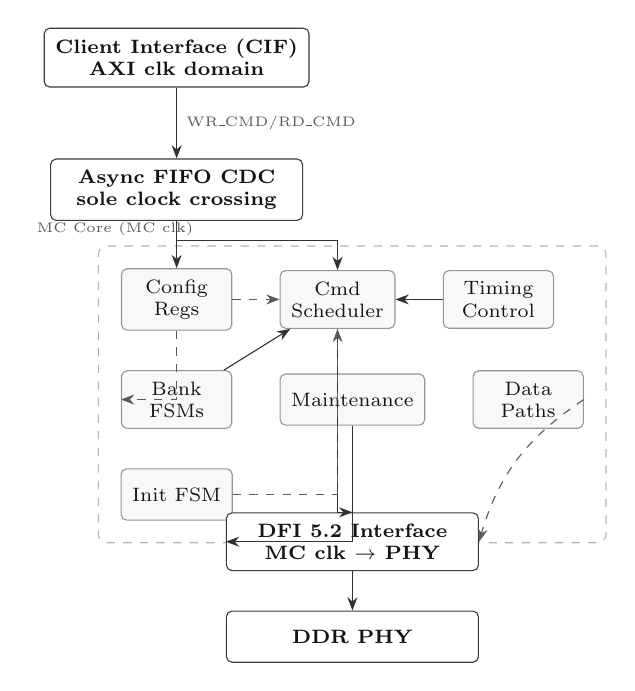
\begin{tikzpicture}[node distance=0.45cm and 1.5cm]
  \node[emblk,minimum width=3.2cm] (cif) {Client Interface (CIF)\\AXI clk domain};
  \node[emblk,minimum width=3.2cm,below=0.9cm of cif] (cdc) {Async FIFO CDC\\sole clock crossing};
  \node[mblk,below=0.6cm of cdc,minimum width=1.4cm] (cfg) {Config\\Regs};
  \node[mblk,right=0.6cm of cfg,minimum width=1.4cm] (sch) {Cmd\\Scheduler};
  \node[mblk,right=0.6cm of sch,minimum width=1.4cm] (tc)  {Timing\\Control};
  \node[mblk,below=0.5cm of cfg,minimum width=1.4cm] (bsm) {Bank\\FSMs};
  \node[mblk,right=0.6cm of bsm,minimum width=1.4cm] (mnt) {Maintenance};
  \node[mblk,right=0.6cm of mnt,minimum width=1.4cm] (dp)  {Data\\Paths};
  \node[mblk,below=0.5cm of bsm,minimum width=1.4cm] (ini) {Init FSM};
  \node[emblk,minimum width=3.2cm,below=1.1cm of mnt] (dfi) {DFI 5.2 Interface\\MC clk $\to$ PHY};
  \node[emblk,minimum width=3.2cm,below=0.5cm of dfi] (phy) {DDR PHY};

  \draw[arr] (cif)--(cdc) node[right,lbl,midway]{WR\_CMD/RD\_CMD};
  \draw[arr] (cdc.south) -- ++(0,-0.25) -| (cfg.north);
  \draw[arr] (cdc.south) -- ++(0,-0.25) -| (sch.north);
  \draw[darr] (cfg)--(sch); \draw[darr] (cfg.south)|-(bsm.west);
  \draw[arr] (bsm)--(sch); \draw[arr] (tc)--(sch);
  \draw[arr] (mnt.south)|-(dfi.west);
  \draw[arr] (sch.south)|-(dfi.north);
  \draw[darr] (ini.east)-|(sch.south);
  \draw[arr] (dfi)--(phy);
  \draw[darr,bend right=20] (dp.east) to (dfi.east);
  \begin{scope}[on background layer]
    \node[grpbox,fit=(cfg)(sch)(tc)(bsm)(mnt)(dp)(ini),
          label={[font=\tiny,color=notetext]above left:MC Core (MC clk)}]{};
  \end{scope}
\end{tikzpicture}
\caption{MC Core top-level architecture. The CDC bar is the sole clock-domain crossing.
         All blocks below it run in the MC clock domain.}
\end{figure}

\subsection{Sub-Block Inventory}

\begin{center}
\begin{tabularx}{\linewidth}{@{} l l X @{}}
\toprule
\Th{Sub-Block} & \Th{Domain} & \Th{Function} \\
\midrule
\RA Config Registers & MC & All timing parameters, page policy, refresh mode, RFM
  thresholds, DFI offsets. Written via AXI4-Lite CSR path. \\
\RB Init FSM & MC & Full DDR5 power-up: RESET\_n, NOP burst, DLL reset, ZQcal
  via MPC, MRW burst, optional training dispatch. Single instance. \\
\RA Bank State Machines & MC & 16 instances, one per bank. Tracks bank state and
  owns all per-bank timers. Source of truth for bank availability. \\
\RB Timing Control & MC & Combinational + registered timer array. Produces
  \texttt{cmd\_ok[15:0][cmd\_type]} each cycle for the Scheduler. \\
\RA Arbitration Logic & MC & Picks winner command class each cycle. Priority,
  age-based anti-starvation, watermark RD/WR mode switching. \\
\RB Command Selector & MC & Takes winner class, applies timing constraints, enforces
  page policy, emits \texttt{\{cmd, rank, BG, bank, row, col\}}. \\
\RA Refresh Scheduler & MC & Leaky-bucket \texttt{tREFI} tracking. REFab and REFsb.
  Up to 8$\times$ postponement; \texttt{ref\_urgent} on overflow. \\
\RB ZQcal FSM & MC & Periodic MPC ZQCAL Start/Latch sequence. \\
\RA RFM FSM & MC & DDR5 rowhammer mitigation. Per-bank RAA counters; triggers
  RFM when RAA $\leq$ RAAIMT. \\
\RB Power Management FSM & MC & CKE-controlled transitions: Active PD, Precharge PD,
  Self-Refresh, MPSM. \\
\RA Write Data Path & MC & BL16-aligned write buffer, DM/ECC generator, Write CRC
  (CRC-8), DFI write timing pipeline. \\
\RB Read Data Path & MC & Read capture FIFO, Read CRC/ECC checker, read latency
  counter, ECS FSM. \\
\bottomrule
\end{tabularx}
\end{center}

%%%%%%%%%%%%%%%%%%%%%%%%%%%%%%%%%%%%%%%%%%%%%%%%%%%%%%%%%%%%%%%%%%%%%%%%%%%%
\section{Config Registers}
%%%%%%%%%%%%%%%%%%%%%%%%%%%%%%%%%%%%%%%%%%%%%%%%%%%%%%%%%%%%%%%%%%%%%%%%%%%%

All timing parameters consumed by the MC Core live here. The host programs them before
asserting \texttt{INIT\_KICK} and may update them at runtime only while the controller is
idle. The Scheduler reads timing values combinatorially every cycle.

\begin{center}
\begin{tabularx}{\linewidth}{@{} l l X @{}}
\toprule
\Th{Register} & \Th{Width} & \Th{Description} \\
\midrule
\RA \texttt{CL} & 7b & CAS Latency (nCK). Drives RL in RTW formula. \\
\RB \texttt{CWL} & 7b & CAS Write Latency $=$ CL$-$2 (fixed in DDR5). \\
\RA \texttt{tRCD} & 8b & RAS-to-CAS delay. ACT to first RD/WR on same bank. \\
\RB \texttt{tRP} & 8b & Row Precharge Time. PRE to next ACT on same bank. \\
\RA \texttt{tRAS} & 9b & Row Active Time minimum. ACT to PRE minimum. \\
\RB \texttt{tRC} & 9b & Row Cycle Time $=$ tRAS$+$tRP. ACT-to-ACT same bank. \\
\RA \texttt{tWR} & 8b & Write Recovery Time. WR burst end to PRE. \\
\RB \texttt{tRTP} & 6b & Read-to-Precharge. RD cmd to PRE on same bank. \\
\RA \texttt{tCCD\_L} & 5b & CAS-to-CAS, same BG (nCK). \\
\RB \texttt{tCCD\_S} & 5b & CAS-to-CAS, diff BG $=$ BL/2 $=$ 8\,nCK. \\
\RA \texttt{tCCD\_L\_WR} & 6b & WR-to-WR same BG. $\max(32\,\text{nCK},\,20\,\text{ns})$. \\
\RB \texttt{tCCD\_L\_WR2} & 6b & WR-to-WR same BG, 2nd not RMW. $\max(16\,\text{nCK},\,10\,\text{ns})$. \\
\RA \texttt{tWTR\_L / tWTR\_S} & 6b/5b & Write-to-Read same/diff BG. \\
\RB \texttt{tRRD\_L / tRRD\_S} & 5b/4b & ACT-to-ACT same/diff BG. \\
\RA \texttt{tFAW} & 6b & Four-Activate Window (nCK). \\
\RB \texttt{tRFC1} & 12b & REFab recovery time. 195\,ns for 8\,Gb DDR5. \\
\RA \texttt{tRFCsb} & 11b & REFsb per-bank recovery time. \\
\RB \texttt{tREFI} & 14b & Average refresh interval. 3.9\,$\mu$s at $\leq$85°C. \\
\RA \texttt{tMRD} & 5b & MRW-to-MRW minimum. 16\,nCK in DDR5. \\
\RB \texttt{tXP / tXS} & 5b/12b & PDX-to-command / SRX-to-command. \\
\RA \texttt{tCKSRE / tCKSRX} & 5b & Stable clock cycles after/before SR entry/exit. \\
\RB \texttt{tDLLK} & 11b & DLL lock time after DLL Reset MPC. 1024\,nCK. \\
\RA \texttt{RAAIMT / RAAMMT} & 8b & RFM RAA Initial/Maximum Management Threshold. \\
\RB \texttt{RAADec} & 4b & RAA decrement per REF command issued. \\
\RA \texttt{REF\_MODE} & 2b & 00=REFab, 01=REFsb, 10=FGR-2$\times$, 11=FGR-4$\times$. \\
\RB \texttt{PAGE\_POLICY} & 2b & 00=Open, 01=Closed, 10=Adaptive. \\
\RA \texttt{AGE\_THR1 / AGE\_THR2} & 8b & Intra/cross-class age escalation thresholds. \\
\RB \texttt{WR\_HIGH\_WM / WR\_LOW\_WM} & 6b & Write pool watermark high/low. \\
\RA \texttt{PHY\_WRLAT / PHY\_RDLAT} & 6b & DFI write/read latency pipeline offsets. \\
\RB \texttt{FREQ\_RATIO} & 2b & DFI frequency ratio: 00=1:1, 01=1:2, 10=1:4. \\
\RA \texttt{INIT\_KICK} & 1b & Write 1 to trigger Init FSM. \\
\RB \texttt{SOFT\_RESET} & 1b & Synchronous soft-reset of all MC Core FSMs. \\
\bottomrule
\end{tabularx}
\end{center}

%%%%%%%%%%%%%%%%%%%%%%%%%%%%%%%%%%%%%%%%%%%%%%%%%%%%%%%%%%%%%%%%%%%%%%%%%%%%
\section{Init FSM}
%%%%%%%%%%%%%%%%%%%%%%%%%%%%%%%%%%%%%%%%%%%%%%%%%%%%%%%%%%%%%%%%%%%%%%%%%%%%

Reference: JESD79-5 \S3.3.1 (power-up with stable power) and \S3.3.2 (reset with stable
power). Single instance. Triggered by \texttt{INIT\_KICK}. Emits DFI commands directly,
bypassing the Cmd Scheduler. Asserts \texttt{init\_done} on completion to release the
Scheduler.

\subsection{State Diagram}

% ── INIT FSM STATE DIAGRAM ───────────────────────────────────────────────────
\begin{figure}[h]
\centering
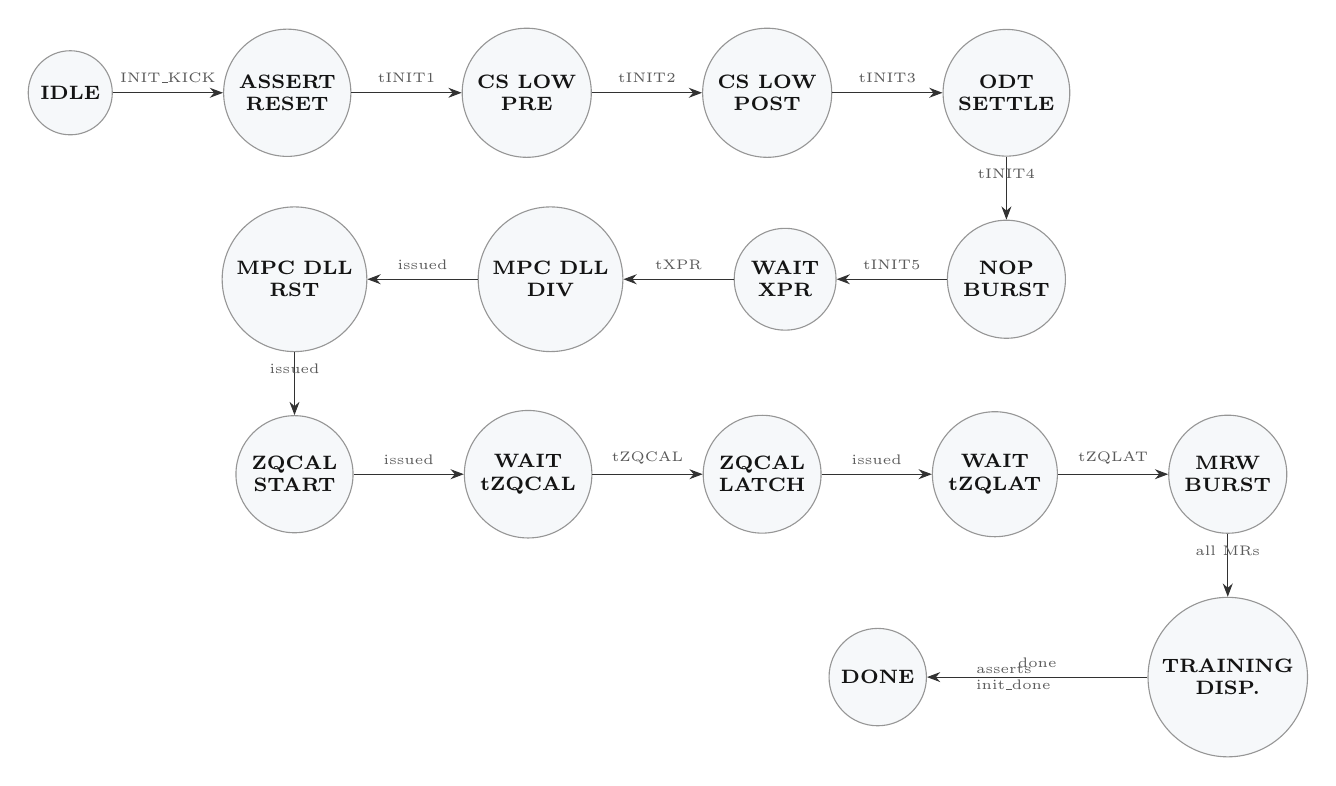
\begin{tikzpicture}[node distance=0.55cm and 1.6cm,
  every node/.style={font=\scriptsize}]

  \node[st,minimum size=0.9cm] (idle)  {IDLE};
  \node[st,minimum size=0.9cm,right=1.4cm of idle]  (rst)  {ASSERT\\RESET};
  \node[st,minimum size=0.9cm,right=1.4cm of rst]   (pre)  {CS LOW\\PRE};
  \node[st,minimum size=0.9cm,right=1.4cm of pre]   (post) {CS LOW\\POST};
  \node[st,minimum size=0.9cm,right=1.4cm of post]  (odt)  {ODT\\SETTLE};
  \node[st,minimum size=0.9cm,below=0.8cm of odt]   (nop)  {NOP\\BURST};
  \node[st,minimum size=0.9cm,left=1.4cm of nop]    (xpr)  {WAIT\\XPR};
  \node[st,minimum size=0.9cm,left=1.4cm of xpr]    (dlld) {MPC DLL\\DIV};
  \node[st,minimum size=0.9cm,left=1.4cm of dlld]   (dllr) {MPC DLL\\RST};
  \node[st,minimum size=0.9cm,below=0.8cm of dllr]  (zqs)  {ZQCAL\\START};
  \node[st,minimum size=0.9cm,right=1.4cm of zqs]   (wzq)  {WAIT\\tZQCAL};
  \node[st,minimum size=0.9cm,right=1.4cm of wzq]   (zql)  {ZQCAL\\LATCH};
  \node[st,minimum size=0.9cm,right=1.4cm of zql]   (wzl)  {WAIT\\tZQLAT};
  \node[st,minimum size=0.9cm,right=1.4cm of wzl]   (mrw)  {MRW\\BURST};
  \node[st,minimum size=0.9cm,below=0.8cm of mrw]   (trn)  {TRAINING\\DISP.};
  \node[st,minimum size=0.9cm,left=2.8cm of trn]    (done) {DONE};

  \foreach \a/\b/\lbl in {
    idle/rst/INIT\_KICK,
    rst/pre/tINIT1,
    pre/post/tINIT2,
    post/odt/tINIT3,
    odt/nop/tINIT4,
    nop/xpr/tINIT5,
    xpr/dlld/tXPR,
    dlld/dllr/issued,
    dllr/zqs/issued,
    zqs/wzq/issued,
    wzq/zql/tZQCAL,
    zql/wzl/issued,
    wzl/mrw/tZQLAT,
    mrw/trn/all MRs,
    trn/done/done}{
    \draw[arr] (\a)--(\b) node[above,lbl,midway]{\lbl};
  }
  % done self-loop note
  \node[right=0.5cm of done,font=\tiny,color=notetext,align=left]
    {asserts\\init\_done};

\end{tikzpicture}
\caption{Init FSM state sequence. Executes once on INIT\_KICK; idles until SOFT\_RESET
         or re-kick. DFI commands issued directly, bypassing Scheduler.}
\end{figure}

\subsection{State Descriptions}

\begin{center}
\begin{tabularx}{\linewidth}{@{} l X l @{}}
\toprule
\Th{State} & \Th{Action} & \Th{Exit Condition} \\
\midrule
\RA IDLE & Hold RESET\_n=0, CKE=0, CS\_n=0. All DFI outputs deasserted. & INIT\_KICK=1 \\
\RB ASSERT\_RESET & RESET\_n held LOW. CS\_n LOW. Load tINIT1 (200\,$\mu$s) counter. & tINIT1 expires \\
\RA CS\_LOW\_PRE & CS\_n LOW. Count tINIT2 (10\,ns) before releasing RESET\_n. & tINIT2 expires \\
\RB CS\_LOW\_POST & Deassert RESET\_n. CS\_n remains LOW. CKE LOW. Count tINIT3 (4\,ms). & tINIT3 expires \\
\RA ODT\_SETTLE & Raise CKE. Stable CK running. Count tINIT4 (2\,$\mu$s). & tINIT4 expires \\
\RB NOP\_BURST & Issue $\geq$3 NOP/DES on DFI. CS\_n driven normally. & tINIT5 NOP count \\
\RA WAIT\_XPR & Count tXPR $=\max(5\,\text{nCK},\,t_{RFC1}+10\,\text{ns})$. & tXPR expires \\
\RB MPC\_DLL\_DIVIDER & Issue MPC: DLL Divider Select (configures tCCD\_L divider via MR13). & cmd accepted \\
\RA MPC\_DLL\_RESET & Issue MPC: DLL Reset. Required before ZQcal. & cmd accepted \\
\RB ZQCAL\_START & Issue MPC opcode ZQCAL Start (OP=0x00). & cmd accepted \\
\RA WAIT\_tZQCAL & Wait. DRAM performs internal ZQ calibration. & 1\,$\mu$s expires \\
\RB ZQCAL\_LATCH & Issue MPC opcode ZQCAL Latch (OP=0x01). & cmd accepted \\
\RA WAIT\_tZQLAT & Wait tZQLAT $=$ 30\,nCK. & tZQLAT expires \\
\RB MRW\_BURST & Issue MRW to MR0, MR2, MR4, MR5, MR6, MR8, MR32--35, MR58. One per tMRD. & all MRWs done \\
\RA TRAINING\_DISPATCH & CA/CS training, Write Leveling, Read training. Controlled by TRAIN\_EN bits. & training done \\
\RB DONE & Assert \texttt{init\_done}. Release Cmd Scheduler from reset. & permanent \\
\bottomrule
\end{tabularx}
\end{center}

\subsection{MRW Sequence}

MR0 (BL, CL), MR2 (2N mode, write leveling), MR4 (refresh/FGR), MR5 (RTT\_PARK, DM),
MR6 (tWR, tRTP), MR8 (BL, preamble, CRC enable), MR32--35 (ODT), MR58 (RFM: read via
MRR, mirror to RAAIMT/RAAMMT config regs). Each write separated by tMRD (16\,nCK).

%%%%%%%%%%%%%%%%%%%%%%%%%%%%%%%%%%%%%%%%%%%%%%%%%%%%%%%%%%%%%%%%%%%%%%%%%%%%
\section{Bank State Machines (BSM)}
%%%%%%%%%%%%%%%%%%%%%%%%%%%%%%%%%%%%%%%%%%%%%%%%%%%%%%%%%%%%%%%%%%%%%%%%%%%%

16 instances, one per bank (2\,BG $\times$ 4\,banks $\times$ 2 sub-channels, or
4\,BG $\times$ 4\,banks for x4/x8 devices). Each BSM is independent, receives commands
from the Cmd Scheduler, and owns all per-bank timers.

\subsection{State Diagram}

% ── BSM STATE DIAGRAM ────────────────────────────────────────────────────────
\begin{figure}[h]
\centering
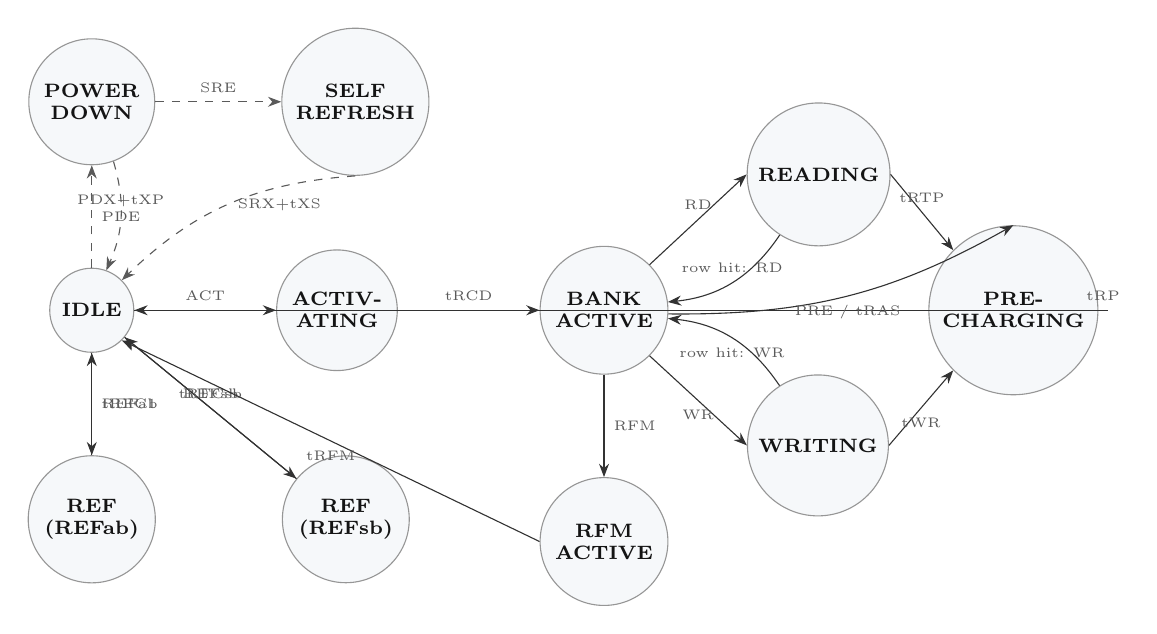
\begin{tikzpicture}[node distance=0.7cm and 1.7cm]

  \node[st] (idle) {IDLE};
  \node[st,right=1.8cm of idle]   (act)  {ACTIV-\\ATING};
  \node[st,right=1.8cm of act]    (ba)   {BANK\\ACTIVE};
  \node[st,above right=0.5cm and 1.5cm of ba] (rd)  {READING};
  \node[st,below right=0.5cm and 1.5cm of ba] (wr)  {WRITING};
  \node[st,right=1.8cm of ba,yshift=0cm,xshift=1.5cm] (pre) {PRE-\\CHARGING};
  \node[st,below=1.3cm of idle]    (ref1) {REF\\(REFab)};
  \node[st,right=1.6cm of ref1]   (ref2) {REF\\(REFsb)};
  \node[st,above=1.3cm of idle]   (pd)   {POWER\\DOWN};
  \node[st,right=1.6cm of pd]     (sr)   {SELF\\REFRESH};
  \node[st,below=1.3cm of ba]     (rfm)  {RFM\\ACTIVE};

  \draw[arr] (idle) -- node[above,lbl]{ACT} (act);
  \draw[arr] (act)  -- node[above,lbl]{tRCD} (ba);
  \draw[arr] (ba.north east) -- node[above,lbl]{RD} (rd.west);
  \draw[arr] (ba.south east) -- node[below,lbl]{WR} (wr.west);
  \draw[arr] (rd.east) -- node[above,lbl]{tRTP} (pre.north west);
  \draw[arr] (wr.east) -- node[below,lbl]{tWR} (pre.south west);
  \draw[arr] (pre) -- node[above,lbl]{tRP} ++(1.2,0) |- (idle.east);
  \draw[arr,bend right=15] (ba) to node[below,lbl]{PRE / tRAS} (pre.north);
  \draw[arr] (idle) -- node[right,lbl]{REFab} (ref1);
  \draw[arr] (idle) -- node[above,lbl]{REFsb} (ref2);
  \draw[arr] (ref1) -- node[right,lbl]{tRFC1} (idle);
  \draw[arr] (ref2) -- node[above,lbl]{tRFCsb} (idle);
  \draw[darr] (idle) -- node[right,lbl]{PDE} (pd);
  \draw[darr] (pd)   to[bend left=20] node[above,lbl]{PDX+tXP} (idle);
  \draw[darr] (pd.east) -- node[above,lbl]{SRE} (sr.west);
  \draw[darr] (sr.south) to[bend right=20] node[right,lbl]{SRX+tXS} (idle.north east);
  \draw[arr] (ba.south) -- node[right,lbl]{RFM} (rfm.north);
  \draw[arr] (rfm.west) -- node[below,lbl]{tRFM} (idle.south east);

  % row hit back-arrows
  \draw[arr,bend left=25] (rd) to node[above,lbl]{\tiny row hit: RD} (ba);
  \draw[arr,bend right=25] (wr) to node[below,lbl]{\tiny row hit: WR} (ba);

\end{tikzpicture}
\caption{Bank State Machine (single bank). 16 instances run independently.
         Dashed arrows: power-state transitions (CKE-controlled).}
\end{figure}

\subsection{State Descriptions}

\begin{center}
\begin{tabularx}{\linewidth}{@{} l l X @{}}
\toprule
\Th{State} & \Th{Legal Inputs} & \Th{Timer / Exit} \\
\midrule
\RA IDLE & ACT, REFab, REFsb, PDE, SRE, RFM & No timer. Exits on received command. \\
\RB ACTIVATING & (internal) & tRCD countdown. Transitions to BANK\_ACTIVE when expired. \\
\RA BANK\_ACTIVE & RD, RDA, WR, WRA, PRE, PREA & tRAS loaded at entry. PRE only after tRAS satisfied. Open row registered. \\
\RB READING & BST (BC8 truncate) & CL+BL/2 until burst end. RDA: hidden PRE starts at tRTP. \\
\RA WRITING & BST (BC8 truncate) & CWL+BL/2 until burst end. WRA: hidden PRE at CWL+BL/2. \\
\RB PRECHARGING & --- & tRP counter. Transitions to IDLE when expired. \\
\RA REFRESHING (REFab) & --- & tRFC1 counter. All 16 banks enter simultaneously. \\
\RB REFRESHING (REFsb) & --- & tRFCsb counter. Only target bank locked; others remain accessible. \\
\RA POWER DOWN & PDX & Precharge PD (from IDLE) or Active PD (from ACTIVE). Exits after PDX+tXP. \\
\RB SELF REFRESH & SRX & tCKSRE after entry. Min tCKESR. SRX: tCKSRX then tXS before commands. \\
\RA RFM ACTIVE & --- & tRFM counter (same duration as tRFC1). Issued by RFM FSM. \\
\bottomrule
\end{tabularx}
\end{center}

\subsection{Per-Bank Timer Summary}

\begin{center}
\begin{tabularx}{0.9\linewidth}{@{} l l X @{}}
\toprule
\Th{Timer} & \Th{Loaded By} & \Th{Guards} \\
\midrule
\RA tRCD & ACT issued & First RD/WR on same bank \\
\RB tRAS & ACT issued & PRE/PREA on same bank (minimum open) \\
\RA tRC & ACT issued & Next ACT on same bank \\
\RB tRP & PRE issued & Next ACT on same bank \\
\RA tWR & WR burst end & PRE on same bank \\
\RB tRTP & RD cmd issued & PRE on same bank \\
\RA tRFC1 & REFab issued & Any command on any bank \\
\RB tRFCsb & REFsb issued & Commands to the refreshed bank only \\
\RA tXS & SRX asserted & First ACT after self-refresh exit \\
\RB tXP & PDX asserted & First command after power-down exit \\
\RA tMRD & MRW issued & Next MRW \\
\bottomrule
\end{tabularx}
\end{center}

%%%%%%%%%%%%%%%%%%%%%%%%%%%%%%%%%%%%%%%%%%%%%%%%%%%%%%%%%%%%%%%%%%%%%%%%%%%%
\section{Timing Control}
%%%%%%%%%%%%%%%%%%%%%%%%%%%%%%%%%%%%%%%%%%%%%%%%%%%%%%%%%%%%%%%%%%%%%%%%%%%%

The Timing Control block is not a state machine. It is a combinational and registered timer
array that produces \texttt{cmd\_ok[15:0][CMD\_TYPES]} every MC clock cycle. The Scheduler
may only issue a command if the corresponding \texttt{cmd\_ok} bit is asserted.

\subsection{Cross-Bank Constraint Checkers}

\begin{center}
\begin{tabularx}{\linewidth}{@{} l l X @{}}
\toprule
\Th{Constraint} & \Th{Scope} & \Th{Implementation} \\
\midrule
\RA tRRD\_L & Same BG, any bank & Timestamp of last ACT in same BG. Block until $T_{now} - T_{last\_ACT\_BG} \geq t_{RRD\_L}$. \\
\RB tRRD\_S & Diff BG, any bank & Timestamp of last ACT globally. Block until $\Delta T \geq t_{RRD\_S}$. \\
\RA tFAW & All banks, same rank & 4-entry ring buffer of recent ACT timestamps. Block if oldest is within tFAW. \\
\RB tCCD\_L & Same BG, RD/WR & Timestamp of last CAS in same BG. \texttt{tCCD\_L\_WR} for WR; \texttt{tCCD\_L\_WR2} for non-RMW. \\
\RA tCCD\_S & Diff BG & Timestamp of last CAS globally. $\Delta T \geq t_{CCD\_S} = $ BL/2. \\
\RB tWTR\_L & Same BG, WR$\to$RD & Last write data end in same BG. Block RD until $\Delta T \geq WL+BL/2+t_{WTR\_L}$. \\
\RA tWTR\_S & Diff BG, WR$\to$RD & Same but using $t_{WTR\_S}$. \\
\RB tRTW & Any, RD$\to$WR & Last RD cmd. Block WR until $\Delta T \geq RL+BL/2 - WL + 2 + t_{WPRE}$. \\
\bottomrule
\end{tabularx}
\end{center}

%%%%%%%%%%%%%%%%%%%%%%%%%%%%%%%%%%%%%%%%%%%%%%%%%%%%%%%%%%%%%%%%%%%%%%%%%%%%
\section{DDR Command Scheduler}
%%%%%%%%%%%%%%%%%%%%%%%%%%%%%%%%%%%%%%%%%%%%%%%%%%%%%%%%%%%%%%%%%%%%%%%%%%%%

The Scheduler is the arbitration heart of the MC Core. It consumes \texttt{cmd\_ok} from
Timing Control, bank states from BSMs, and pending transactions from the RD/WR Cmd Pools.
It issues one DFI command per clock cycle.

\subsection{Scheduler FSM}

% ── SCHEDULER FSM ────────────────────────────────────────────────────────────
\begin{figure}[h]
\centering
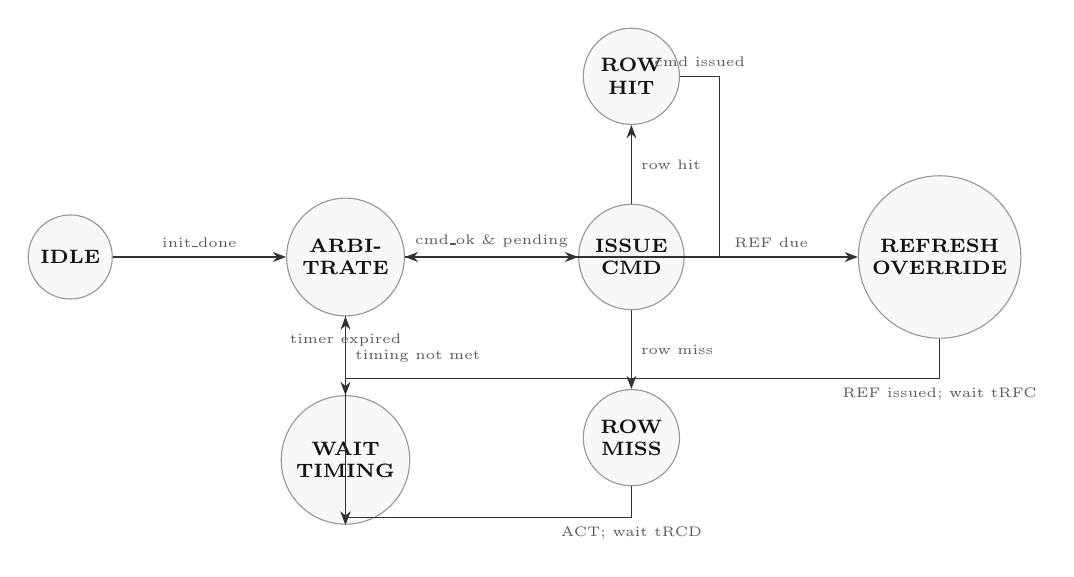
\begin{tikzpicture}[node distance=0.8cm and 2.0cm]
  \node[st] (idle)  {IDLE};
  \node[st,right=2.2cm of idle]  (arb)   {ARBI-\\TRATE};
  \node[st,right=2.2cm of arb]   (issue) {ISSUE\\CMD};
  \node[st,below=1.0cm of arb]   (wait)  {WAIT\\TIMING};
  \node[st,above=1.0cm of issue] (hit)   {ROW\\HIT};
  \node[st,below=1.0cm of issue] (miss)  {ROW\\MISS};
  \node[st,right=2.2cm of issue] (ref)   {REFRESH\\OVERRIDE};

  \draw[arr] (idle) -- node[above,lbl]{init\_done} (arb);
  \draw[arr] (arb)  -- node[above,lbl]{cmd\_ok \& pending} (issue);
  \draw[arr] (arb)  -- node[right,lbl]{timing not met} (wait);
  \draw[arr] (wait) -- node[above,lbl]{timer expired} (arb);
  \draw[arr] (issue.north) -- node[right,lbl]{row hit} (hit.south);
  \draw[arr] (issue.south) -- node[right,lbl]{row miss} (miss.north);
  \draw[arr] (hit.east)  -| node[above,lbl,near start]{cmd issued} ++(0.5,0) |- (arb.east);
  \draw[arr] (miss.south) -- ++(0,-0.4) node[below,lbl]{ACT; wait tRCD} -| (wait.south);
  \draw[arr] (issue.east) -- node[above,lbl]{REF due} (ref);
  \draw[arr] (ref.south)  -- ++(0,-0.5) node[below,lbl]{REF issued; wait tRFC} -| (wait.south);
\end{tikzpicture}
\caption{DDR Command Scheduler FSM. One command issued per MC clock cycle.}
\end{figure}

\subsection{Command Priority Order}

\begin{enumerate}
  \item Refresh Override --- REF budget about to expire (highest priority)
  \item RFM --- RAA $\leq$ RAAIMT (safety critical)
  \item ZQcal --- periodic, low urgency until overdue
  \item Write drain --- write buffer nearly full
  \item Row-hit reads --- open page, same row
  \item Row-hit writes
  \item Row-miss reads --- ACT $\to$ wait tRCD $\to$ RD
  \item Row-miss writes
  \item PRE --- close idle banks if closed-page policy active
\end{enumerate}

\subsection{Page Policy}

\begin{center}
\begin{tabularx}{\linewidth}{@{} l l l X @{}}
\toprule
\Th{Policy} & \Th{Row Hit} & \Th{Row Miss} & \Th{Best For} \\
\midrule
\RA Open Page & CAS only & PRE $\xrightarrow{t_{RP}}$ ACT $\xrightarrow{t_{RCD}}$ CAS & Sequential, high spatial locality \\
\RB Closed Page & ACT+CAS (always) & ACT $\xrightarrow{t_{RCD}}$ CAS & Random access; streaming workloads \\
\RA Adaptive & Hit-rate decides & Sliding window $N=256$ & Mixed; autotunes per bank independently \\
\bottomrule
\end{tabularx}
\end{center}

Adaptive thresholds: hit\_rate $>$ OPEN\_THR (default 70\%) $\Rightarrow$ open;
hit\_rate $<$ CLOSE\_THR (default 30\%) $\Rightarrow$ closed.

\subsection{Arbitration Logic}

Runs every MC clock. Selects the winning command class. Does not select bank/row/col --- that is
the Command Selector's job.

\textbf{Priority hierarchy:}

\begin{center}
\begin{tabularx}{\linewidth}{@{} c l l X @{}}
\toprule
\Th{Level} & \Th{Winner} & \Th{Condition} & \Th{Effect} \\
\midrule
\RA 0 & REF urgent & Credits $\geq 8$ or $\Delta t_{since\_REF} > t_{REFI\_max}$ & Hard stall; all RD/WR suppressed \\
\RB 1 & REF nominal & tREFI countdown reaches zero & REF injected; RD/WR deferred \\
\RA 2 & ZQ calibration & tZQCS interval expires & ZQCS after current REF completes \\
\RB 3 & Read & RD pool non-empty \& RD mode active & BG-aware scheduling \\
\RA 4 & Write & WR pool non-empty \& WR mode active & Watermark-controlled batching \\
\RB 5 & Scrubber/MRR & Background maintenance, idle slot & Pre-emptible \\
\bottomrule
\end{tabularx}
\end{center}

\textbf{Age counter (anti-starvation):} Every RD/WR pool entry carries an age counter incremented
each MC cycle. At AGE\_THR1 (default 64): intra-class head-of-line bypass. At AGE\_THR2
(default 256): WR entry may overtake RD priority. Age resets to 0 on dispatch.

\textbf{RD/WR mode switching:} Switch to WR mode when WR depth $\geq$ WR\_HIGH\_WM (32) or RD
empty. Switch back when WR depth $\leq$ WR\_LOW\_WM (8) or WR empty or urgent RD.
Hysteresis gap of 24 entries prevents mode thrashing.

\subsection{Command Selector --- Legal Check Matrix}

All gates must be true before dispatch. Any false $\Rightarrow$ NOP inserted.

\begin{center}
\begin{tabularx}{\linewidth}{@{} l l X @{}}
\toprule
\Th{Gate} & \Th{Timer Source} & \Th{Constraint} \\
\midrule
\RA \texttt{bank\_avail[b]} & BSM state & Bank not in ACTIVATING or PRECHARGING \\
\RB \texttt{gate\_rcd[b]} & ACT issue & $t_{RCD}$: ACT to first CAS on same bank \\
\RA \texttt{gate\_rp[b]} & PRE issue & $t_{RP}$: PRE to ACT on same bank \\
\RB \texttt{gate\_ras[b]} & ACT issue & $t_{RAS}$: ACT to PRE minimum \\
\RA \texttt{gate\_ccd\_l} & Same BG CAS & $t_{CCD\_L}$ or $t_{CCD\_L\_WR}$ or $t_{CCD\_L\_WR2}$ \\
\RB \texttt{gate\_ccd\_s} & Diff BG CAS & $t_{CCD\_S} = $ BL/2 \\
\RA \texttt{gate\_rrd\_l} & Same BG ACT & $t_{RRD\_L}$ \\
\RB \texttt{gate\_rrd\_s} & Diff BG ACT & $t_{RRD\_S}$ \\
\RA \texttt{gate\_faw} & Sliding window & $\leq$4 ACTs within $t_{FAW}$ \\
\RB \texttt{gate\_wtr\_l} & WR data end, same BG & $t_{WTR\_L}$: WR to RD \\
\RA \texttt{gate\_wtr\_s} & WR data end, diff BG & $t_{WTR\_S}$: WR to RD \\
\RB \texttt{gate\_rtw} & RD cmd & $t_{RTW} = RL + BL/2 + 2 - WL$ \\
\RA \texttt{gate\_rfc[r]} & REF issue, per rank & $t_{RFC1}$: all commands blocked \\
\RB \texttt{gate\_rfcpb[r][b]} & REFsb, per bank & $t_{RFCsb}$: same bank only blocked \\
\RA \texttt{gate\_zqcs} & ZQCS issue & All commands blocked during ZQ \\
\RB \texttt{gate\_mrd} & MRW issue & $t_{MRD}$: MRW to MRW \\
\bottomrule
\end{tabularx}
\end{center}

%%%%%%%%%%%%%%%%%%%%%%%%%%%%%%%%%%%%%%%%%%%%%%%%%%%%%%%%%%%%%%%%%%%%%%%%%%%%
\section{Maintenance Engine}
%%%%%%%%%%%%%%%%%%%%%%%%%%%%%%%%%%%%%%%%%%%%%%%%%%%%%%%%%%%%%%%%%%%%%%%%%%%%

Four independent sub-FSMs handle all autonomous background operations. Each posts requests
to the Cmd Scheduler via a priority request bus.

\subsection{Refresh Scheduler FSM}

States: IDLE $\to$ REF\_DUE $\to$ WAIT\_BANKS\_IDLE $\to$ ISSUE\_REF $\to$ WAIT\_tRFC
$\to$ DONE $\to$ IDLE. REFsb path substitutes WAIT\_TARGET\_BANK\_IDLE and WAIT\_tRFCsb.

\begin{itemize}
  \item \textbf{Leaky-bucket counter:} increments by 1 each $t_{REFI}$. Decrements on REF issued.
        If counter reaches 9: \texttt{ref\_urgent} asserted, hard-stalling all RD/WR.
  \item \textbf{REFsb cycling:} bank address cycles BA[1:0] in order $00 \to 01 \to 10 \to 11$.
        8 REFsb commands $\approx$ 1 REFab credit.
  \item \textbf{FGR mode:} REF\_MODE[1]=1 $\Rightarrow$ tRFC2; REF\_MODE[1:0]=11 $\Rightarrow$ tRFC4.
        Budget counter threshold halved or quartered.
  \item \textbf{Temperature derating:} MR4 TUF=1 $\Rightarrow$ tREFI halved before loading into
        credit tracker. MC polls MR4 periodically via background MRR.
\end{itemize}

\subsection{ZQcal FSM}

States: IDLE $\to$ WAIT\_IDLE $\to$ ISSUE\_ZQCAL\_START $\to$ WAIT\_tZQCAL $\to$
ISSUE\_ZQCAL\_LATCH $\to$ WAIT\_tZQLAT $\to$ DONE $\to$ IDLE.

Triggered by periodic tZQCS interval timer (CSR-configurable) or host write to
\texttt{ZQCAL\_TRIG}. All banks must be idle before issuing. During ZQCAL, all commands
blocked via \texttt{gate\_zqcs}. tZQCAL = 1\,$\mu$s; tZQLAT = 30\,nCK.

\subsection{RFM FSM (Rowhammer Management)}

States: IDLE $\to$ MONITOR\_RAA $\to$ RFM\_REQUEST $\to$ WAIT\_ISSUE $\to$ WAIT\_tRFM
$\to$ UPDATE\_RAA $\to$ MONITOR\_RAA.

RAA counter logic:
\begin{itemize}
  \item RAA[b] $+= 1$ on every ACT to bank $b$.
  \item RAA[b] $-=$ RAADec on every REF issued to bank $b$.
  \item RAA[b] $\leq$ RAAIMT: assert RFM request to Scheduler (priority: above ZQcal, below refresh override).
  \item tRFM $=$ tRFC1 (same duration). Bank enters RFM\_ACTIVE during this window.
  \item After tRFM: RAA[b] reset. Return to MONITOR\_RAA.
\end{itemize}

\subsection{Power Management FSM}

States: NORMAL $\to$ PD\_ENTRY\_CHECK $\to$ \{PRECHARGE\_PD or ACTIVE\_PD\} $\to$
PDX\_WAIT\_tXP $\to$ NORMAL. Self-Refresh branch: NORMAL $\to$ SR\_ENTRY $\to$
WAIT\_tCKSRE $\to$ SELF\_REFRESHING $\to$ SR\_EXIT $\to$ WAIT\_tCKSRX $\to$
WAIT\_tXS $\to$ WAIT\_tDLLK $\to$ NORMAL.

\begin{itemize}
  \item \textbf{Precharge PD:} from IDLE. All banks idle. CKE deasserted.
  \item \textbf{Active PD:} from BANK\_ACTIVE. Bank retains open row. Resumes after PDX+tXP.
  \item \textbf{Self-Refresh:} all banks precharged first. tCKSRE after CKE falls. On SRX:
        tCKSRX stable clock, then tXS, then tDLLK.
  \item \textbf{MPSM:} MR2 OP[1:0]=01. Deeper than SR. Exit via DES then MRW to clear MPSM.
\end{itemize}

%%%%%%%%%%%%%%%%%%%%%%%%%%%%%%%%%%%%%%%%%%%%%%%%%%%%%%%%%%%%%%%%%%%%%%%%%%%%
\section{Write Data Path}
%%%%%%%%%%%%%%%%%%%%%%%%%%%%%%%%%%%%%%%%%%%%%%%%%%%%%%%%%%%%%%%%%%%%%%%%%%%%

\begin{center}
\begin{tabularx}{\linewidth}{@{} l X @{}}
\toprule
\Th{Sub-Block} & \Th{Description} \\
\midrule
\RA Write Data Buffer & BL16-aligned FIFO. Stores write data from CIF Write Cmd Pool via CDC FIFO.
  Dequeued when Scheduler confirms a write slot. \\
\RB DM/ECC Generator & Computes per-byte Data Mask. Generates inline Write CRC using CRC-8
  polynomial $G(x) = x^4 + x + 1$ over DQ+DM bits per BL16 burst.
  Write CRC enabled via MR8 OP[6]=1. \\
\RA WL Align & Inserts programmable pipeline delay $=$ CWL nCK to align DQS preamble to
  \texttt{dfi\_wrdata\_en}. Offset from PHY\_WRLAT config reg. \\
\RB DFI Write Timing & Drives \texttt{dfi\_wrdata[127:0]}, \texttt{dfi\_wrdata\_mask[15:0]},
  \texttt{dfi\_wrdata\_cs\_n}, \texttt{dfi\_parity\_in}. Preamble per MR8 (2\,tCK default).
  ODT timing: $t_{ODTon}=WL-2$, $t_{ODToff}=WL+BL/2$. \\
\RA Write CRC Error FSM & States: NORMAL $\to$ CRC\_ERROR\_DETECTED $\to$ RETRY\_WRITE $\to$
  AUTO\_DISABLE. Monitors \texttt{dfi\_alert\_n}. Retries up to $n$ times (MR51/52).
  Auto-disables Write CRC via MRW to MR8 if threshold exceeded. \\
\bottomrule
\end{tabularx}
\end{center}

%%%%%%%%%%%%%%%%%%%%%%%%%%%%%%%%%%%%%%%%%%%%%%%%%%%%%%%%%%%%%%%%%%%%%%%%%%%%
\section{Read Data Path}
%%%%%%%%%%%%%%%%%%%%%%%%%%%%%%%%%%%%%%%%%%%%%%%%%%%%%%%%%%%%%%%%%%%%%%%%%%%%

\begin{center}
\begin{tabularx}{\linewidth}{@{} l X @{}}
\toprule
\Th{Sub-Block} & \Th{Description} \\
\midrule
\RA Read Latency Counter & Per-outstanding-read counter. Tracks CL + read preamble cycles from
  RD command issue to expected data arrival. Issues \texttt{dfi\_rddata\_en} exactly
  PHY\_RDLAT cycles before expected \texttt{dfi\_rddata\_valid}. \\
\RB Read Data FIFO & Captures \texttt{dfi\_rddata[127:0]} when \texttt{dfi\_rddata\_valid}
  asserts. Re-aligns per-burst data. Feeds CIF Reorder Buffer with AXI transaction tag. \\
\RA ECC/CRC Checker & Verifies Read CRC when MR8 OP[7]=1. On error: flags to CIF error register,
  optionally triggers read retry. Read CRC adds latency adder to RL (JESD79-5 Table 365). \\
\RB ECS FSM & States: IDLE $\to$ ECS\_ACTIVE $\to$ WAIT\_tECS $\to$ IDLE. Triggered by
  MR14 (auto-ECS) or host MPC request. DRAM scrubs on-die ECC during tECS window
  ($\leq t_{RFC1}$). Error logs in MR16--MR20. \\
\bottomrule
\end{tabularx}
\end{center}

%%%%%%%%%%%%%%%%%%%%%%%%%%%%%%%%%%%%%%%%%%%%%%%%%%%%%%%%%%%%%%%%%%%%%%%%%%%%
\section{DFI 5.2 Interface}
%%%%%%%%%%%%%%%%%%%%%%%%%%%%%%%%%%%%%%%%%%%%%%%%%%%%%%%%%%%%%%%%%%%%%%%%%%%%

DFI timing: \texttt{dfi\_wrdata\_en} asserted PHY\_WRLAT cycles before write data.
\texttt{dfi\_rddata\_valid} arrives PHY\_RDLAT cycles after the RD command.
Both offsets are PHY-specific and set during DFI training. FREQ\_RATIO determines
nCK per DFI clock.

\begin{center}
\begin{tabularx}{\linewidth}{@{} l l X @{}}
\toprule
\Th{Signal} & \Th{Dir} & \Th{Description} \\
\midrule
\RA \texttt{dfi\_address[13:0]} & MC$\to$PHY & CA bus. 2-cycle encoding for DDR5 ACT. \\
\RB \texttt{dfi\_cs\_n[1:0]} & MC$\to$PHY & Chip select per rank. \\
\RA \texttt{dfi\_cke[1:0]} & MC$\to$PHY & Clock Enable per rank. \\
\RB \texttt{dfi\_odt[1:0]} & MC$\to$PHY & On-Die Termination control per rank. \\
\RA \texttt{dfi\_reset\_n} & MC$\to$PHY & DRAM RESET\_n. Driven by Init FSM. \\
\RB \texttt{dfi\_act\_n} & MC$\to$PHY & Activate indicator (DDR5). \\
\RA \texttt{dfi\_bank[1:0]} & MC$\to$PHY & Bank address. \\
\RB \texttt{dfi\_bg[2:0]} & MC$\to$PHY & Bank group. BG[2:0] for x4/x8; BG[1:0] for x16. \\
\RA \texttt{dfi\_wrdata[127:0]} & MC$\to$PHY & Write data (BL16 $\times$ DQ8 per sub-channel). \\
\RB \texttt{dfi\_wrdata\_mask[15:0]} & MC$\to$PHY & Write data mask per byte lane. \\
\RA \texttt{dfi\_wrdata\_en} & MC$\to$PHY & Asserted PHY\_WRLAT cycles early. \\
\RB \texttt{dfi\_wrdata\_cs\_n} & MC$\to$PHY & Per-DRAM write chip select (DDR5 PDA). \\
\RA \texttt{dfi\_parity\_in} & MC$\to$PHY & CA parity bit (DDR5). \\
\RB \texttt{dfi\_rddata[127:0]} & PHY$\to$MC & Captured read data. \\
\RA \texttt{dfi\_rddata\_valid} & PHY$\to$MC & Read data valid flag. \\
\RB \texttt{dfi\_rddata\_dnv} & PHY$\to$MC & Data-not-valid error flag. \\
\RA \texttt{dfi\_alert\_n} & PHY$\to$MC & DRAM alert: Write CRC or CA parity error. \\
\RB \texttt{dfi\_ctrlupd\_req/ack} & MC$\leftrightarrow$PHY & Controller-initiated PHY update handshake. \\
\RA \texttt{dfi\_phyupd\_req/ack} & PHY$\leftrightarrow$MC & PHY-initiated update/pause handshake. \\
\RB \texttt{dfi\_init\_start/complete} & MC$\leftrightarrow$PHY & Init FSM PHY initialization handshake. \\
\RA \texttt{dfi\_freq\_ratio[1:0]} & MC$\to$PHY & 00=1:1, 01=1:2, 10=1:4. \\
\bottomrule
\end{tabularx}
\end{center}

%%%%%%%%%%%%%%%%%%%%%%%%%%%%%%%%%%%%%%%%%%%%%%%%%%%%%%%%%%%%%%%%%%%%%%%%%%%%
\section{FSM Inventory}
%%%%%%%%%%%%%%%%%%%%%%%%%%%%%%%%%%%%%%%%%%%%%%%%%%%%%%%%%%%%%%%%%%%%%%%%%%%%

\begin{center}
\begin{tabularx}{0.9\linewidth}{@{} l r r X @{}}
\toprule
\Th{FSM} & \Th{States} & \Th{Instances} & \Th{Notes} \\
\midrule
\RA Init FSM & 16 & 1 & RESET\_n through training complete \\
\RB Bank State Machine & 11 & 16 & One per bank; 176 total state bits \\
\RA Arbitration Logic & 6 & 1 & RD/WR mode + priority selection \\
\RB Command Selector & 4 & 1 & Page policy + legal check + sequence gen \\
\RA Refresh Scheduler & 7 & 1 & REFab + REFsb + FGR + urgent override \\
\RB ZQcal FSM & 7 & 1 & MPC ZQCAL Start/Latch flow \\
\RA RFM FSM & 6 & 1 & Per-bank RAA monitoring + RFM injection \\
\RB Power Management FSM & 10 & 1 & PD (Pre/Act), SR, MPSM \\
\RA Write CRC Error FSM & 4 & 1 & \texttt{dfi\_alert\_n} monitoring; retry + auto-disable \\
\RB ECS FSM & 4 & 1 & DDR5 inline ECC scrub window \\
\midrule
\RA \textbf{Total} & \textbf{$\approx$75} & \textbf{23} & \\
\bottomrule
\end{tabularx}
\end{center}

%%%%%%%%%%%%%%%%%%%%%%%%%%%%%%%%%%%%%%%%%%%%%%%%%%%%%%%%%%%%%%%%%%%%%%%%%%%%
\section{Timing Reference}
%%%%%%%%%%%%%%%%%%%%%%%%%%%%%%%%%%%%%%%%%%%%%%%%%%%%%%%%%%%%%%%%%%%%%%%%%%%%

Reference values at 200\,MHz (tCK=5\,ns, CL=3, CWL=1, BL/2=8) and 100\,MHz (tCK=10\,ns).
Production values set via Config Regs from actual speed bin.

\begin{center}
\begin{tabularx}{\linewidth}{@{} l l r r @{}}
\toprule
\Th{Command Sequence} & \Th{Formula} & \Th{@200\,MHz} & \Th{@100\,MHz} \\
\midrule
\RA ACT $\to$ RD/WR (same bank) & tRCD & 4 & 4 \\
\RB ACT $\to$ PRE (same bank, min) & tRAS & 7 & 4 \\
\RA PRE $\to$ ACT (same bank) & tRP & 4 & 4 \\
\RB ACT $\to$ ACT (same bank) & tRC = tRAS+tRP & 11 & 8 \\
\RA ACT $\to$ ACT (same BG) & tRRD\_L & 4 & 4 \\
\RB ACT $\to$ ACT (diff BG) & tRRD\_S & 2 & 2 \\
\RA RD $\to$ RD (same BG) & tCCD\_L & 8 & 8 \\
\RB WR $\to$ WR (same BG) & tCCD\_L\_WR & 32 & 32 \\
\RA WR $\to$ WR same BG (not RMW) & tCCD\_L\_WR2 & 16 & 16 \\
\RB RD/WR (diff BG) & tCCD\_S = BL/2 & 8 & 8 \\
\RA RD $\to$ WR (any) & RL+BL/2$-$WL+2+tWPRE & 14 & 14 \\
\RB WR $\to$ RD (same BG) & WL+BL/2+tWTR\_L & 13 & 13 \\
\RA WR $\to$ RD (diff BG) & WL+BL/2+tWTR\_S & 11 & 11 \\
\RB REFab $\to$ any & tRFC1 & 39 & 20 \\
\RA SRX $\to$ ACT & tXS = tRFC1+10\,ns & 41 & 21 \\
\RB ZQCAL Start $\to$ Latch & tZQCAL = 1\,$\mu$s & 200 & 100 \\
\RA 4 ACT window & tFAW & 16 & 16 \\
\bottomrule
\end{tabularx}
\end{center}

%%%%%%%%%%%%%%%%%%%%%%%%%%%%%%%%%%%%%%%%%%%%%%%%%%%%%%%%%%%%%%%%%%%%%%%%%%%%
\section{DDR5 vs DDR4 --- Design Deltas}
%%%%%%%%%%%%%%%%%%%%%%%%%%%%%%%%%%%%%%%%%%%%%%%%%%%%%%%%%%%%%%%%%%%%%%%%%%%%

\begin{center}
\begin{tabularx}{\linewidth}{@{} l l X @{}}
\toprule
\Th{Feature} & \Th{DDR4} & \Th{DDR5 --- MC Core Impact} \\
\midrule
\RA BL & BL8 (BL/2=4) & BL16 (BL/2=8). All RTW, WTR, WR-to-PRE formulae scale by 2. \\
\RB ACT encoding & 1-cycle CA & 2-cycle CA. Scheduler drives CA on two consecutive rising edges. \\
\RA REFsb & Not supported & Refresh Scheduler adds REFsb path; per-bank tRFCsb timer in BSM. \\
\RB RFM & Not supported & Full RFM FSM; per-bank RAA counters; RAAIMT/RAAMMT in Config Regs. \\
\RA ZQ mechanism & ZQCL/ZQCS commands & MPC ZQCAL Start+Latch. Init FSM restructured; ZQcal FSM uses MPC. \\
\RB tRFC1 (8\,Gb) & 350\,ns & 195\,ns. Shorter penalty; more scheduling headroom. \\
\RA tREFI & 7.8\,$\mu$s & 3.9\,$\mu$s. Double refresh rate; budget counter threshold halved. \\
\RB CWL & Separate lookup & CWL = CL$-$2 (fixed). Simplifies Config Reg and RTW formula. \\
\RA tMOD & 24\,nCK after MRS & Replaced by tMRD only (16\,nCK). No separate tMOD path. \\
\RB tCCD\_L\_WR & Not defined & $\max(32\,\text{nCK},\,20\,\text{ns})$. New gate in Command Selector. \\
\RA Write CRC & Optional (MR5) & Mandatory support. \texttt{dfi\_alert\_n} monitoring; Write CRC Error FSM. \\
\RB ECS & Not supported & ECS FSM in Read Data Path; hooks into tRFC window. \\
\RA MR addressing & 3 MRs & 256 MRs (MR0--MR255) via MRW/MRR. Init FSM MRW burst extended. \\
\bottomrule
\end{tabularx}
\end{center}

\vspace{10pt}
\noindent\color{ruleclr}\rule{\linewidth}{0.4pt}\\[2pt]
{\small\color{notetext}
MC Core Design Specification --- Memory Controller Capstone Project.
JEDEC JESD79-5 (DDR5) / DFI\,5.2 / AXI4. Timing values device-specific;
validate against datasheet for each speed bin.}

\end{document}
